% Copyright 2021 Joel Feldman, Andrew Rechnitzer and Elyse Yeager, except where noted.
% This work is licensed under a Creative Commons Attribution-NonCommercial-ShareAlike 4.0 International License.
% https://creativecommons.org/licenses/by-nc-sa/4.0/


%----------------------------------------------------------------------------------------
\section*{0.6: Inverse Functions}

\begin{frame}{Table of Contents \hfill\only<beamer>{\hyperlink{210ln}{\beamerskipbutton{Skip review of inverse functions and logarithms}}}}
\renewcommand{\invf}{highlightcolor}
\mapofcontentsBB{}
\renewcommand{\invf}{C2!30}
\end{frame}
 
%----------------------------------------------------------------------------------------
\note{\scriptsize Students are often scared of inverse trig functions and logarithms, so I carve out time to talk about inverse functions in general, and those inverse functions in particular. We start with a game: I know $y$, you guess $x$. I take time to make sure students are comfortable with the game, because we'll use it later with logarithms. Having this intuitive understanding seems really helpful. Again, this takes time, but for me it's been a good investment. Otherwise many students muddle through memorizing $\ln 1 = 0$ and occasionally misremembering it as $\ln 0 = 1$ with no foundation to decide which one is correct.

I make the game into silly fun. Write my $x$ down so they know I'm not lying, but for things like $\sin x=0$, make it unguessable -- like $-12,501\pi$. Either have the whole class shout out guesses, or have one brave volunteer join you at the front for a few rounds. Candy as a reward for correct guesses. 

One year I taught two classes, and someone from the first class warned someone in the second class that I was writing down 72$\pi$, so someone in the second class raised their hand to guess that was what I had written down. I had written down something else, but I wish I'd kept it the same. Imagine the class's reaction if that guess had been correct!}
%-------------------------------------------------------------
%---------------------------------------

\begin{frame}[t]{Invertibility Game}

\begin{itemize}[<+->]
	\item A function $y=f(x)$ is known to both players
	\item \textcolor{M4}{Player A} chooses a secret value $x$ in the domain of $f(x)$
	\item \textcolor{M4}{Player A} tells \textcolor{M3}{Player B} what $f(x)$ is
	\item \textcolor{M3}{Player B} tries to guess \textcolor{M4}{Player A}'s $x$-value.
\end{itemize}\pause\vfill
\begin{center}
	\textbf{Round 1:} $f(x)=2x$
	\pause\vfill
	\textbf{Round 2:} $f(x)=\sqrt[3]{x}$
	\pause\vfill
	\textbf{Round 3:} $f(x)=|x|$
	\pause\vfill
	\textbf{Round 4:} $f(x)=\sin x$
	\vfill
\end{center}
\note<5>{``I'm thinking of a value of $x$. $f(x)=10$ for this $x$. What $x$ am I thinking of?" etc.}
\note<6>{For $f(x)=|x|$, the first guesses are usually the negative of what you said. So if you say ``I'm thinking of an $x$, and $f(x)$ is 9, the first guesses tend to be $-9$. So I usually write down $x=9$ on my secret paper. (We're trying to introduce the idea that sometimes you can't necessarily guess right, so I want students to get it wrong. But there will be more opportunities.)}
\end{frame}
%-------------------------------------------------------------
%----------------------------------------------------------------------------------------
%----------------------------------------------------------------------------------------
\begin{frame}{Functions are Maps}
\note<1>{A visual model for what we're doing is helpful because it helps students to generalize the ideas. For the examples where they compute inverses, I think students tend to do their inverting ad-hoc. That makes it hard to talk about inverses in general, because they don't have a picture in their mind of a generic function inversion.}
\begin{center}\begin{tikzpicture}
\draw (0,0) node[shape=ellipse, minimum width=3cm, minimum height=5cm, draw]{};
\draw (0,3) node{domain}; 
\draw (5,0) node[shape=ellipse, minimum width=3cm, minimum height=5cm, draw]{};
\draw (5,3) node{range}; 
\draw[->, ultra thick, C2] (1,2) to[out=45, in=135] (4,2);
\draw[C2] (2.5,2) node{$f(x)=\sqrt[3]{x}$};

\iftoggle{printsolutions}{
	
	\draw (0,.5) node(a1){8};
	\draw (5,.5) node(b1){2};
	\draw (0,-.5) node(c1){27};
	\draw (5,-.5) node(d1){3};
	\draw (0,-1.5) node(e1){-1};
	\draw (5,-1.5) node(f1){-1};
	\onslide<2>{
		\draw[C2, thick, ->] (a1)--(b1);
		\draw[C2, thick, ->] (e1)--(f1);
		\draw[C2, thick, ->] (c1)--(d1);}
	\onslide<4->{
		\draw[M3, thick, <-] (a1)--(b1);
		\draw[M3, thick, <-] (e1)--(f1);
		\draw[M3, thick, <-] (c1)--(d1);}
}{}

\onslide<5->{
	\draw[ultra thick, M3, <-] (1,-2) to[out=-45, in=-135] (4,-2);
	\draw[M3] (2.5,-2) node{$f^{-1}(x)=x^3$};}
\end{tikzpicture}\end{center}
\unote{Definition~\eref{text}{def inv func}}
\end{frame}
%----------------------------------------------------------------------------------------
%----------------------------------------------------------------------------------------
\begin{frame}{Functions are Maps}
\begin{center}
\begin{tikzpicture}
\draw (0,0) node[shape=ellipse, minimum width=3cm, minimum height=5cm, draw]{};
\draw (0,3) node{domain}; 
\draw (5,0) node[shape=ellipse, minimum width=3cm, minimum height=5cm, draw]{};
\draw (5,3) node{range}; 
\draw[->, ultra thick, C2] (1,2) to[out=45, in=135] (4,2);
\draw[C2] (2.5,2) node{$f(x)=|x|$};

\iftoggle{printsolutions}{

\draw (0,.5) node(a1){0};
\draw (5,.5) node(b1){0};
\draw (0,-.5) node(c1){2};
\draw (5,-.5) node(d1){2};
\draw (0,-1.5) node(e1){-2};

\onslide<2>{
	\draw[C2, thick, ->] (a1)--(b1);
	\draw[C2, thick, ->] (c1)--(d1);
	\draw[C2, thick, ->] (e1)--(d1);}
\onslide<4->{
	\draw[M3, thick, ->] (b1)--(a1);
	\draw[M3, thick, ->] (d1)--(.75,-1)node[left]{??};}
}{}

\onslide<5->{
\draw[ultra thick, M3, <-] (1,-2) to[out=-45, in=-135] (4,-2);
\draw[M3] (2.5,-2) node{$f^{-1}(x)$ DNE};}
\end{tikzpicture}
\end{center}

\end{frame}
%----------------------------------------------------------------------------------------
\begin{frame}[t]
\note<1>{Students have now seen two ways of thinking of inverses: the invertibility game, and thinking of functions as a map. The horizontal line test is still difficult for them, because it's another step of transference. They'll be able to state it and use it if you just \textit{tell} it to them, but many won't understand it unless you really take a few minutes to give examples. When there's a function that fails the horizontal line test, play the invertibility game. ``I pick this $y$, can you tell me which $x$ I'm thinking of?" Accompany that with a horizontal line through all points on the function that have the same $y$-value, and many students will come up with the horizontal line test for themselves.}
\begin{center}
\begin{tikzpicture}
\myaxis{x}{3}{3}{y}{3}{3}
\onslide<1-4|handout:1-2>{\draw[ultra thick, C2] plot[domain=-2.8:2.8](\x,{\x});}

\onslide<3-4|handout:2>{
\draw (1,1) node[shape=circle, minimum size=2mm, draw, C2, inner sep=0, fill=white]{};
\draw (1,2) node[shape=circle, minimum size=2mm, fill, C2, inner sep=0]{};}

\onslide<5-6|handout:3>{\draw[ultra thick, C2] plot[domain=0:2.8](\x,{.6*(\x*\x-4)});
\draw[C2] (-1.5,1.5) node{$x^2-4$, $x\geq 0$};}

\end{tikzpicture}

\vfill
\hfill 
\alert<2,6|handout:0>{A. invertible} \hfill 
\alert<4|handout:0>{B. not invertible} \hfill ~
\end{center}
\only<1,3,5>{\AnswerYes}
\note<6>{When students specifically see the quadratic function, they often jump to ``not invertible" because of the $x^2$ term. Restricting the domain is important, because it allows us to defined e.g. arcsine.  So I linger here a while, and play the inverse game a few times. ``Could I have been thinking of -1? No, because that's not allowed by the restricted domain."}

\unote{Definition~\eref{text}{def_0_6_2}}
\end{frame}
%----------------------------------------------------------------------------------------
\begin{frame}[t]{Relationship between $f(x)$ and $f^{-1}(x)$}
\note<1>{Option D is to make sure everyone participates. If a lot of students aren't raising their hands for any option, have them chat with their neighbours for a minute, then try again.

With the visual explanation, I've found saying ``for example, suppose $f(x)=x^3$" and using numbers works somehow better than having ``$x$" on the left and ``$y$" or ``$f(x)$" on the right.}

Let $f$ be an invertible function.

What is $f^{-1}(f(x))$?

\begin{itemize}
\alert<3-|handout:0>{\item[A.] $x$}
\item[B.] $1$
\item[C.] $0$
\item[D.] not sure
\end{itemize}

\onslide<2-3|handout:0>{
\hfill\begin{tikzpicture}
\draw (0,0) node[shape=ellipse, minimum width=2cm, minimum height=3cm, draw,label=above:{domain}](D){};
\draw (5,0) node[shape=ellipse, minimum width=2cm, minimum height=3cm, draw,label=above:{range}](R){};



\draw (D) node(d){125};
\draw (R) node(r){5};

\draw[C2, thick, ->] (d) to[bend left] (r);
\draw[C2] ($(D)!0.5!(R)$)+(0,1.5) node{$f(x)$};

\draw[M3, thick, <-] (d) to[bend right] (r);
\draw[M3]  ($(D)!0.5!(R)$)+(0,-1.5)  node{$f^{-1}(x)$};
\end{tikzpicture}}

\end{frame}
%----------------------------------------------------------------------------------------
\begin{frame}[t]
\only<4>{\QuestionBar{1}{3}\AnswerYes}
\only<5>{\QuestionBar{2}{3}\AnswerYes}
\only<6>{\QuestionBar{3}{3}\AnswerYes}
\note<1>{Again, students will easily remember the rule ``swap $x$ and $y$ and solve for $y$," but concrete examples help them understand why it works: an inverse function swaps the role of output ($y$) and input ($x$).

If you want students to calculate the first on on their own (ie before they've explicitly seen an example of how to do this for something they can't do in their heads), remind them of the invertibility game. I'm thinking of an $x$, and $f(x)=3$. What is $x$? This is the cue to set up $f(x)=3$ and solve for $x$.}
\note<6>{\small ``Rather than do this every time we want to play the game, let's solve the game once and for all. No matter WHAT number I tell you, find a function that will let you know what you should guess as the answer." 

Many will initially write $f(x)=x$, and many will be able to solve it just fine by remembering that the two $x$'s mean different things. Point out that they mean different things. In the language of the game, $x$ is what I (teacher) say, $y$ is what they (students) say. We're treating the information I give them as the input, because it's the thing they start out knowing.

This will be hard for many students, which is why we're spending so much time on it.}
\begin{block}{Invertibility}
In order for a function to be invertible \pause,
different $x$ values cannot map to the same $y$ value.\pause

We call such a function \textbf{one-to-one}, or
\textbf{injective}.
\end{block}
\pause

Suppose $f(x)=\sqrt[3]{19+x^3}$. What is $f^{-1}(3)$? (simplify your answer)

\iftoggle{printsolutions}{\onslide<7>{\alert{$f(2)=3$, so $f^{-1}(3)=2$}}}{}\vfill
\pause

What is $f^{-1}(10)$? (do not simplify) \pause

\iftoggle{printsolutions}{\onslide<7>{\alert{$\sqrt[3]{19+y^3}=10$ tells us $f^{-1}(10)=\sqrt[3]{10^3-19}$}}}{}\vfill

What is $f^{-1}(x)$?

\iftoggle{printsolutions}{\onslide<7>{\alert{$\sqrt[3]{19+y^3}=x$ tells us $f^{-1}(x)=\sqrt[3]{x^3-19}$}}}{}\vfill

\unote{Definition~\eref{text}{def_0_6_1}}
\end{frame}
%------------------------------------------------------------------
%----------------------------------------------------------------------------------------
\begin{frame}[t]
\begin{center}Let $f(x)=x^2-x$.\end{center}
\vfill
1. Sketch a graph of $f(x)$, and choose a (large) domain over which it is invertible.
\vfill

2. For the domain you chose, evaluate $f^{-1}(20)$.
\vfill

3. For the domain you chose, evaluate $f^{-1}(x)$.
\vfill 

4. What are the domain and range of $f^{-1}(x)$? What are the (restricted) domain and range of $f(x)$?
\vfill

\AnswerYes\MoreSpace
\end{frame}
%----------------------------------------------------------------------------------------
\begin{frame}[t]
\note<1>{``One option is ... / Another option is ..."\\

When going through the computations, point out what the answer is for students who chose the other domain. Otherwise is can be stressful for those students.}
\begin{tikzpicture}[yscale=0.9]
\onslide<-6>{\myaxis{x}{1.5}{2.5}{y}{.5}{4}}
\onslide<8-|handout:0>{\myaxis{a}{1.5}{2.5}{b}{.5}{4}}
\draw[C1, very thick] plot[domain=-1.5:2.5,smooth](\x,{\x*\x-\x})node[right]{\only<-6>{$y=x^2-x$}\only<8-|handout:0>{$b=a^2-a$}};
\answer{\onslide<2>{\fill[pattern=horizontal lines dark gray,opacity=0.75] (2.5,-.5) rectangle (.5,4);
	\draw (.5,-1)node[left]{Domain: $\left(-\infty,\tfrac12\right]$};}
	\onslide<3->{\fill[pattern=horizontal lines dark gray,opacity=0.75] (-1.55,-.4) rectangle (.5,3.9);}
	\onslide<3-4>{\draw (1.5,-1)node[right]{Domain: $\left[\tfrac12,\infty\right)$};}
	\onslide<5->{\ycoord[fill=white]{2}{\only<-6>{20}\only<9->{x}}
	\xcoord{2}{\only<-6>{f^{-1}(20)}\only<9>{f^{-1}(x)}\only<10>{\frac{1+\sqrt{1+4x}}{2}}}
	\draw[thick,white] (0,2)-|(2,0);\draw[dashed] (0,2)-|(2,0);}
}
\end{tikzpicture}

\answer{
	\abovedisplayskip=-2em
	\only<4-6>{\color{answercolor}
	\begin{align*}
	\color{black}{f^{-1}(20)=}\onslide<6>{5 &&\\
	&&20&=x^2-x\\
	&&0&=x^2-x-20 = (x-5)(x+4)\\
	&&x&=5}
	\end{align*}}
	\only<7->{\color{answercolor}
		\begin{align*}
		\color{black}f^{-1}(x)= \onslide<10->{\tfrac{1+\sqrt{1+4x}}{2}& &a^2-a &= x \mbox{, find $a$}\\
		&&a^2-a-x&=0\\
		&&a&=\tfrac{1 \pm \sqrt{1+4x}}{2}\\
		&&f^{-1}(x)&=\tfrac{1+\sqrt{1+4x}}{2}}
		\end{align*}
	}
}
\end{frame}
%----------------------------------------------------------------------------------------
\begin{frame}[t]
\onslide<3-|handout:0>{\color{C2}$f(x) = x^2-x,$ domain: $\left[\frac{1}{2},\infty\right)$}
\onslide<6-|handout:0>{\hfill \color{M3} $f^{-1}(x) = \tfrac{1+\sqrt{1+4x}}{2}$}

\begin{center}\begin{tikzpicture}
\draw[black] (0,0) node[shape=ellipse, minimum width=3cm, minimum height=5cm, draw]{};
\draw[C2] (0,3) node{domain of $f(x)$}; 
\draw[black] (5,0) node[shape=ellipse, minimum width=3cm, minimum height=5cm, draw]{};
\draw[C2] (5,3) node{range of $f(x)$}; 
\draw[->, ultra thick, C2] (1,2) to[out=45, in=135] (4,2);
\draw[C2] (2.5,2) node{$f(x)$};
\draw[ultra thick, M3, <-] (1,-2) to[out=-45, in=-135] (4,-2);
\draw[M3] (2.5,-2.) node{$f^{-1}(x)$};

\onslide<2-|handout:0>{
\draw[M3] (0,-3) node{range of $f^{-1}(x)$}; 
\draw[M3] (5,-3) node{domain of $f^{-1}(x)$}; }

\onslide<4-|handout:0>{\draw[black] (0,0) node{$\left[\frac{1}{2},\infty \right)$};}
\onslide<5-|handout:0>{\draw[black] (5,0) node{$\left[-\frac{1}{4},\infty \right)$};}
\end{tikzpicture}\end{center}
\end{frame}

%----------------------------------------------------------------------------------------
\section{A.13 Logarithms}
%----------------------------------------------------------------------------------------
%----------------------------------------------------------------------------------------
%\begin{frame}[t]{Invertibility game: $f(x)=e^x$}
%
%\begin{itemize}[<+->]
%	\item I'm thinking of an $x$. Your clue: $f(x)=e$. What is my $x$?\vfill
%	\item I'm thinking of an $x$. Your clue: $f(x)=1$. What is my $x$?\vfill
%	\item I'm thinking of an $x$. Your clue: $f(x)=\frac1e$. What is my $x$?\vfill
%	\item I'm thinking of an $x$. Your clue: $f(x)=e^3$. What is my $x$?\vfill
%	\item I'm thinking of an $x$. Your clue: $f(x)=0$. What is my $x$?\vfill
%\end{itemize}
%
%\end{frame}
%------------------------------------------------------------------
%----------------------------------------------------------------------------------------
\begin{frame}[t]{Invertibility game: $f(x)=e^x$ \hfill \onslide<7->{\textcolor{C3}{$f^{-1}(x)=\log_e x$}}}
\begin{itemize}[<+->]
	\item I'm thinking of an $x$. Your clue: $f(x)=e$. What is my $x$?
	\onslide<6-|handout:0>{\alert{$x=1$}} \\\hfill\onslide<8-|handout:0>{\textcolor{C3}{$\log_e(e)=1$}}
	\vfill
	\item I'm thinking of an $x$. Your clue: $f(x)=1$. What is my $x$?
	\onslide<6-|handout:0>{\alert{$x=0$}}\\\hfill\onslide<8-|handout:0>{\textcolor{C3}{$\log_e(1)=0$}}
	\vfill
	\item I'm thinking of an $x$. Your clue: $f(x)=\frac1e$. What is my $x$?
	\onslide<6-|handout:0>{\alert{$x=-1$}}\\\hfill\onslide<8-|handout:0>{\textcolor{C3}{$\log_e\left(\tfrac1e\right)=-1$}}
	\vfill
	\item I'm thinking of an $x$. Your clue: $f(x)=e^3$. What is my $x$?
	\onslide<6-|handout:0>{\alert{$x=3$}}\\\hfill\onslide<8-|handout:0>{\textcolor{C3}{$\log_e(e^3)=3$}}
	\vfill
	\item I'm thinking of an $x$. Your clue: $f(x)=0$. What is my $x$?
	\onslide<6-|handout:0>{\alert{Trick question: no $x$ gives $f(x)=0$.}}
	\\\hfill\onslide<8-|handout:0>{\textcolor{C3}{$\log_e(x)$ is undefined at $x=0$}}\vfill
\end{itemize}
\only<1-5,7>{\AnswerYes}
\end{frame}
%---------------------------------------------------------------------------------------
%------------------------------------------------------------------
\begin{frame}[t]
\begin{enumerate}
\item Suppose $0<x<1$. Then $\log_e (x)$ is...
\vfill
\item Suppose $-1<x<0$. Then $\log_e (x)$ is...
\vfill
\item Suppose $e<x$. Then $\log_e (x)$ is...
\end{enumerate}\vfill
\begin{enumerate}[A.]\centering
\item positive\item negative \item greater than one \item less than one \item undefined
\end{enumerate}
\AnswerNo
\end{frame}
%------------------------------------------------------------------
\begin{frame}[t]{Exponents and Logarithms}
\centering
\abovedisplayskip=0pt
\[f(x) = e^x \hspace{2cm} f^{-1}(x) =\log_e(x)=\ln (x) \textcolor{M5}{ =\log(x)}\]\pause

\begin{tabular}{c c | c | c c}
\textbf{$x$}&\textbf{$e^x$}&\onslide<3->{ \textbf{$e$} fact $\leftrightarrow$ $\log_e$ fact & $x$ & $\log_e (x)$} \\
\hline
$0$&$1$&\onslide<4-|handout:0>{ $e^{\alert{0}}=1~\leftrightarrow~\log_e(1)=\alert{0}$ & 1 & 0}\\
$1$&$e$& \onslide<5-|handout:0>{ $e^{\alert{1}}=e~\leftrightarrow~\log_e(e)=\alert{1}$& $e$ & 1 }\\
$-1$&$\frac{1}{e}$& \onslide<6-|handout:0>{  $e^{\alert{-1}}=\frac{1}{e}~\leftrightarrow~\log_e(\frac{1}{e})=\alert{-1}$
& $\frac1e$ & $-1$}\\
$n$&$e^n$& \onslide<7-|handout:0>{$e^{\alert{n}}=e^n~\leftrightarrow~\log_e(e^n)=\alert{n}$ & $e^n$ & $n$  }
\end{tabular}\vfill
\end{frame}
%------------------------------------------------------------------
\begin{frame}
\begin{center}
\begin{tikzpicture}[scale=0.9]
\myaxis{x}{5}{5}{y}{4}{4}

\draw[C2, ultra thick] plot[domain=-5:1.5, samples=50] (\x,{exp(\x)}) node[right]{$y=e^x$}; 
\draw[M3, ultra thick] plot[domain=.03:5, samples=100] (\x,{ln(\x)}) node[above]{$y=\log_e(x)$}; 

\answer{\onslide<2-7>{
\draw[C2] (0,1) node[vertex] (a){};
\draw[C2] (a) node[left]{$(0,1)$};
}

\onslide<3-7>{
\draw[M3] (1,0) node[vertex] (a1){};
\draw[M3] (a1) node[below right]{$(1,0)$};
}


\onslide<4-7>{
\draw[C2] (1,2.7) node[vertex] (b){};
\draw[C2] (b) node[left]{$(1,e)$};
}

\onslide<5-7>{
\draw[M3] (2.7,1) node[vertex] (b1){};
\draw[M3] (b1) node[below right]{$(e,1)$};
}

\onslide<6-7>{
\draw[C2] (-1,.37) node[vertex] (c){};
\draw[C2] (c) node[above left]{$(-1,1/e)$};
}

\onslide<7-7>{
\draw[M3] (.37,-1) node[vertex] (c1){};
\draw[M3] (c1) node[below right]{$(1/e,-1)$};
}

\onslide<8->{
\draw[dashed, thick] plot[domain=-4:4] (\x,{\x}) node[right] {$y=x$};}
}
\end{tikzpicture}\end{center}
\end{frame}
%-------------------------------------------------------------
\begin{frame}[t]{Logs of Other Bases: $\log_n(x)$ is the inverse of $n^x$}
$\log_{10} 10^8=$
\begin{itemize}
\item[A.] 0
\item[B.] 8 \iftoggle{printsolutions}{\onslide<2->{$\checkmark$}}{}
\item[C.] 10
\item[D.] other
\end{itemize}\pause\pause\vfill

$\log_{2} 16 = $
\begin{itemize}
\item[A.] 1
\item[B.] 2
\item[C.] 3
\item[D.] other
 \iftoggle{printsolutions}{ \onslide<4->{$\checkmark$ \color{M4} $2^4=16$ so $\log_2 16 = 4$}}{}
\end{itemize}\vfill

\end{frame}

%------------------------------------------------------------------
\begin{frame}[t]
\begin{block}{Logarithm Rules}
\note<1>{Pause after each slide is to let you derive the rules}
Let $A$ and $B$ be positive, and let $n$ be any real number.\pause

{$\log(A \cdot B) = \pause \log(A)+ \log(B)$\\}
{\textcolor{answercolor}{Proof:  $\log(A \cdot B) = \log(e^{\log A}e^{\log B})=\log(e^{\log A+\log B})=\log(A)+\log(B)$
\vfill}}\pause

{$\log(A/B) =\pause \log(A)-\log(B)$\\
\textcolor{answercolor}{Proof: $\log(A/B) = \log\left(\frac{e^{\log A}}{e^{\log B}}\right) = \log(e^{\log A - \log B}) = \log A - \log B$ 
\vfill}}\pause

{$\log (A^n) \pause = n\log (A)$}\\
\textcolor{answercolor}{Proof: $\log(A^n)=\log\left(\left(e^{\log A}\right)^n\right)=\log\left(e^{n\log A}\right)=n\log A$}
\end{block}
\end{frame}
%------------------------------------------------------------------
\begin{frame}[t]
\begin{block}{Logarithm Rules}
Let $A$ and $B$ be positive, and let $n$ be any real number.

$\log(A \cdot B) =  \log(A)+ \log(B)$\\
$\log(A/B) = \log(A)-\log(B)$\\
$\log (A^n)  = n\log (A)$\\
\end{block}\pause

\vspace{.3cm}
\only<2>{Write as a single logarithm:\\ $f(x) = \log\left(\dfrac{10}{x^2} \right)+2\log x+\log(10+x)$\AnswerYes}\pause
\color{answercolor}
\answer{
\abovedisplayskip=-1em
\begin{align*}
f(x) &= \log\left(\tfrac{10}{x^2} \right)+2\log x+\log(10+x)\\
&=\log 10 -\log (x^2)+2\log x + \log (10+x)\\
&= \log 10 -2\log x +2\log x + \log (10+x)\\
&= \log 10 + \log (10+x)
= \log (10(10+x)))\\
&=\log (100+10x)
\end{align*}}
\end{frame}
%----------------------------------------------------------------------------------------
\begin{frame}[t]{Base Change}
\begin{align*}
\mbox{Fact:} \qquad b^{\log_b(a)}&=a\\
\onslide<2->{\Rightarrow \log \big(b^{\log_b(a)}\big)&=\log(a)\\
\Rightarrow \log_b(a)\log (b)&=\log(a)\\
\Rightarrow \log_b(a) &= \frac{\log(a)}{\log (b)}}
\end{align*}
\onslide<3->{In general, for positive $a$, $b$, and $c$:
\[\boxed{\log_b(a) = \frac{\log_c(a)}{\log_c(b)}}\]}
\end{frame}
%----------------------------------------------------------------------------------------
\begin{frame}[t]
In general, for positive $a$, $b$, and $c$:
\[\boxed{\log_b(a) = \frac{\log_c(a)}{\log_c(b)}}\]
\vfill
Suppose your calculator can only compute logarithms base 10. What would you enter to calculate $\log(17)$?
\onslide<2-|handout:0>{\alert{$\frac{\log_{10}(17)}{\log_{10}(e)}$}}
\vfill
Suppose your calculator can only compute natural logarithms. What would you enter to calculate $\log_2(57)$?
\onslide<2-|handout:0>{\alert{$\frac{\log(57)}{\log(2)}$}}
\vfill
Suppose your calculator can only compute logarithms base 2. What would you enter to calculate $\log(2)$?
\onslide<2-|handout:0>{\alert{$\frac{\log_2 2}{\log_{2}e} = \frac{1}{\log_2 e}$}}
\only<1>{\AnswerYes}
\end{frame}
%----------------------------------------------------------------------------------------
\mode<beamer>{\begin{frame}
\begin{multicols}{2}
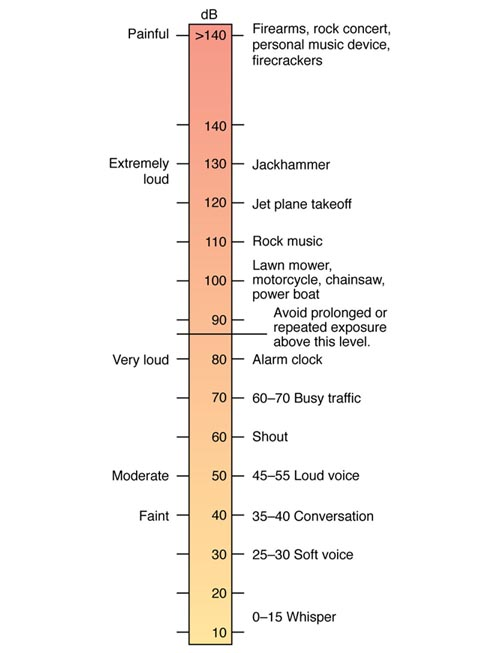
\includegraphics[height=.9\textheight]{Clipart/decibels.jpeg}
\index{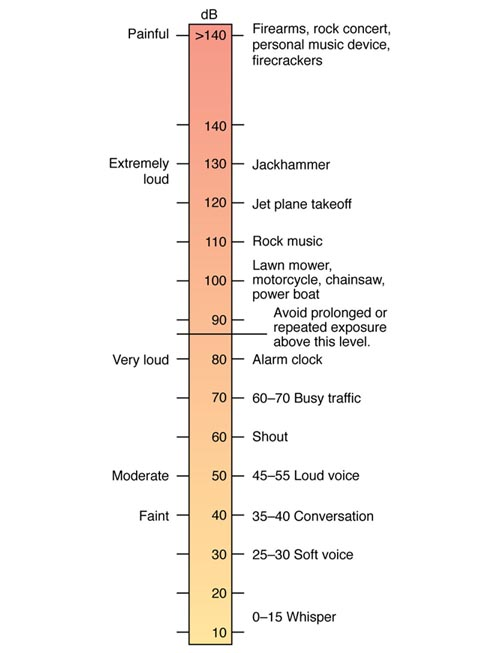
\includegraphics[height=10mm]{Clipart/decibels.jpeg}  \parbox[b]{.8\textwidth}{\raggedright Anonymous.  (2012)  \href{http://biology-forums.com/index.php?action=gallery;sa=view;id=6156}{Decibel Scale of Frequently Heard Sounds}. Biology Forums. \url{http://biology-forums.com/index.php?action=gallery;sa=view;id=6156} (accessed 7 October 2015)}}
\columnbreak

Decibels: For a particular measure of the power $P$ of a sound wave, the decibels of that sound is:
\[10\log_{10}(P)\]
So, every ten decibels corresponds to a sound being ten \textbf{times} louder.\vfill
\end{multicols}
\end{frame}}
%------------------------------------------------------------------
\begin{frame}
\only<1>{\AnswerYes}
Decibels: For a particular measure of the power $P$ of a sound wave, the decibels of that sound is:
\[10\log_{10}(P)\]
So, every ten decibels corresponds to a sound being ten \textbf{times} louder.\vfill

\color{C1}A lawnmower emits a 100dB sound. How much sound will two lawnmowers make?
\begin{itemize}
	\item[A.] 100 dB
	\item[B.] 110 dB
	\item[C.] 200 dB
	\item[D.] other \iftoggle{printsolutions}{\only<2-|handout:0>{$\checkmark$ \color{M4}more than 100, less than 110}}{}
\end{itemize}
\end{frame}

%----------------------------------------------------------------------------------------
\section*{2.10: Natural Log}

\begin{frame}{Table of Contents}\label{210ln}
\mapofcontentsBB{\bk}
\end{frame}

%-------------------------------------------------------------
\begin{frame}[t]{Differentiating the Natural Logarithm}
Calculate $\diff{}{x}\{\log_e x\}$.\pause

\only<-3>{
	One Weird Trick:
\begin{align*}
x&=e^{\log_e x}\\ 
\onslide<3>{
\diff{}{x}\{x\}&=\diff{}{x}\left\{e^{\log_e x}\right\}\\
1&=e^{\log_e x}\cdot\diff{}{x}\{\log_e x\}=x\cdot\diff{}{x}\{\log_e x\}\\
\frac{1}{x}&=\diff{}{x}\{\log_e x\}
}
\end{align*}}
\only<4-|handout:0>{\begin{block}{Derivative of Natural Logarithm -- Theorem~\eref{text}{thm diff log}}
		\[\ds\diff{}{x}\{\log_e x\}=\dfrac{1}{x}\qquad(x>0)\]
		
		\onslide<5->{\[\diff{}{x}\left\{\log_e|x|\right\}=\onslide<6->{\frac{1}{x}\qquad(x \neq 0)}\]}
\end{block}}

\end{frame}
%-------------------------------------------------------------
%------------------------------------------------------------------
\note{``We showed it for $\ln x$ and $x>0$, but it works the same for $\ln (-x)$ and $x<0$"}
%----------------------------------------------------------------------------------------
\begin{frame}[t]
\begin{block}{Derivative of Natural Logarithm}
\[\diff{}{x}\left\{\log_e|x|\right\}=\frac{1}{x}\qquad(x \neq 0)\]
\end{block}


Differentiate: $f(x) = \log_e |x^2+1|$ \pause

\color{M4}
\iftoggle{printsolutions}{
We use the chain rule:
\begin{align*}
\diff{}{x}\left\{\log_e \left|\boxed{x^2+1}\right|\right\} & = 
\frac{1}{x^2+1} \cdot\left(2x\right)\\
&=\frac{2x}{x^2+1}
\end{align*}
}{}
\end{frame}

%%%%%%%%%%%%%%%%%%%%%%%%%%%%%%%%%%%%%%%%%%%%%%

%----------------------------------------------------------------------------------------
\begin{frame}[t]
\note<1>{We'll re-do derivs of logs (including with abs values) in 2.11 using implicit differentiation}
\begin{block}{Derivatives of Logarithms -- Corollary~\eref{text}{cor_2_10}}
For $a>0$:
\[\diff{}{x}[\log_a|x|] = \frac{1}{x\log a}\]\\$ $\\

In particular:
\[\diff{}{x}[\log |x|] = \frac{1}{x}\]
\end{block}\pause


Differentiate: $f(x) = \log_e |\cot x|$ \pause
\color{answercolor}

\answer{We use the chain rule:
\begin{align*}
\diff{}{x}[\log_e \left|\boxed{\cot x}\right|] & = 
\frac{1}{\cot x} \cdot \big(-\csc^2x\big)=\frac{-\csc^2x}{\cot x}
\end{align*}}
\end{frame}
%----------------------------------------------------------------------------------------
%\begin{frame}[t]
%\only<1>{\QuestionBar{1}{5}\AnswerYes}
%\only<2>{\AnswerBar{1}{5}}
%\[f(x) = \frac{(x^2+17)(32x^{10}-8)}{\sin x +2}\]
%\vfill\pause
%\answer{\color{answercolor}\scriptsize\vspace{-5mm}
%\begin{align*}
% \frac{(x^2+17)(32x^{10}-8)}{\sin x +2}&=y\\
% \ln \left|  \frac{(x^2+17)(32x^{10}-8)}{\sin x +2}\right|&=\ln |y|&\ln\mbox{ both sides}\\
%\ln |x^2+17|+\ln |32x^{10}-8|-\ln |\sin x +2|&=\ln|y|&\mbox{ log rules}\\
%\diff{}{x}\left[\ln |x^2+17|+\ln |32x^{10}-8|-\ln |\sin x +2|\right]&=\diff{}{x}[\ln|y|]&\mbox{differentiate}\\
%\frac{2x}{x^2+17}+
%\frac{320x^9}{32x^{10}-8}-\frac{\cos x}{\sin x}&=
%\frac{y'}{y}\\
%y\left(\frac{2x}{x^2+17}+
%\frac{320x^9}{32x^{10}-8}-\frac{\cos x}{\sin x+2}\right)
%&=y'\\
%\left(\frac{2x}{x^2+17}+
%\frac{320x^9}{32x^{10}-8}-\frac{\cos x}{\sin x+2} \right)
%\cdot \frac{(x^2+17)(32x^{10}-8)}{\sin x +2}&=y'&\mbox{ plug in $y$}
%\end{align*}}
%\end{frame}
%----------------------------------------------------------------------------------------

\begin{frame}{Logarithmic Differentiation - A Fancy Trick}
\begin{itemize}
\item $\log(f\cdot g) = \log f + \log g$\\
\vfill\onslide<2->{multiplication turns into addition}
\vfill
\item $\log\left(\frac{f}{g} \right) = \log f- \log g$
\vfill\onslide<2->{division turns into subtraction}
\vfill
\item $\log\left(f^g \right)=g\log f$
\vfill\onslide<2->{exponentiation turns into multiplication}
\vfill
\onslide<3->{\alert{We can exploit these properties to differentiate!}}
\end{itemize}
\end{frame}
%----------------------------------------------------------------------------------------
\begin{frame}[t]
\begin{block}{Logarithmic Differentiation}
In general, if $f(x)\neq 0$, $\diff{}{x}\left[\log|f(x)| \right] = \frac{f'(x)}{f(x)}$.
\end{block}
\[f(x)=\left(
\frac{(2x+5)^4(x^2+1)}{x+3}
\right)^5\]

Find $f'(x)$.\\ \vfill

\note<1>{``Slide rules made use of logarithm properties to make other (non-logarithmic) computations faster. " Note this trick works well when functions are sums, products, and powers of other functions.}
\only<1|handout:0>{\hfill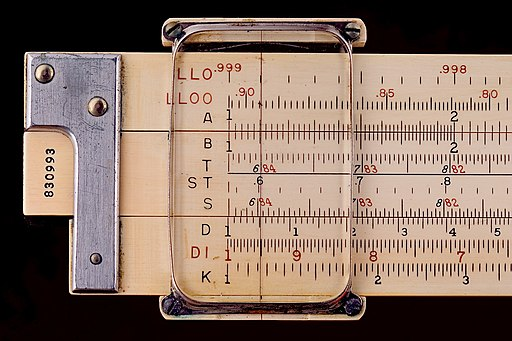
\includegraphics[height=3cm]{Clipart/slide.jpg}

\index{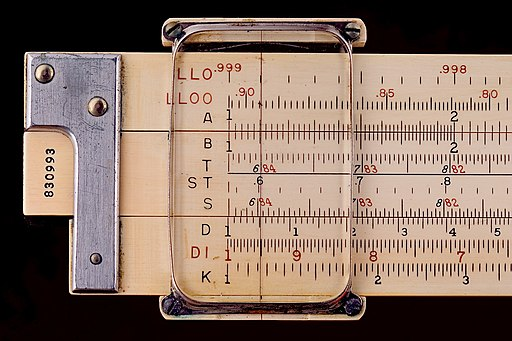
\includegraphics[height=5mm]{Clipart/slide.jpg}~\parbox[b]{.8\textwidth}{\raggedright
\href{https://commons.wikimedia.org/wiki/File:Keuffel_&_Esser_slide_rule,_model_4081-3_(ca._1940)_-_Detail.jpg}{`Slide rule -- KEUFFEL \& ESSER CO. N.Y. ' } by
\href{https://www.flickr.com/people/45032885\%40N04}{s58y}
is licensed under \CCBYtwo~ (accessed 20 July 2021)
}}

\MoreSpace\AnswerYes}
\unote{Example~\eref{text}{eg_2_10_4}}
\end{frame}
%----------------------------------------------------------------------------------------
%----------------------------------------------------------------------------------------
\begin{frame}[t]{Logarithmic Differentiation - A Fancy Trick}
\only<1>{\QuestionBar{1}{5}\AnswerYes}
\only<2>{\AnswerBar{1}{5}}
\note<1>{Space given after equals sign to take ln of both sides}
\[f(x)=\qquad\left(
\frac{(2x+5)^4(x^2+1)}{x+3}
\right)^5\]\pause
\color{answercolor}\iftoggle{printsolutions}{

\begin{align*}
\log(f(x))&=\log\left[
\left(
\frac{(2x+5)^4(x^2+1)}{x+3}
\right)^5
\right]\\
&=5\log\left[
\frac{(2x+5)^4(x^2+1)}{x+3}
\right]
\\&=5\Big[4\log\left(
2x+5\right)+\log(x^2+1)-\log(x+3)
\Big]\\
\frac{f'(x)}{f(x)}&=5\left[4\frac{2}{2x+5}+\frac{2x}{x^2+1}-\frac{1}{x+3}
\right]\\
f'(x)&= \left(
\frac{(2x+5)^4(x^2+1)}{x+3}
\right)^5\cdot
5\left[4\frac{2}{2x+5}+\frac{2x}{x^2+1}-\frac{1}{x+3}
\right]
\end{align*}
}{}
\end{frame}
%----------------------------------------------------------------------------------------
\begin{frame}[t]{Logarithmic Differentiation - A Fancy Trick}
\only<1>{\QuestionBar{2}{5}\AnswerYes}
\only<2>{\AnswerBar{2}{5}}
\note<1>{Students will desperately want to do power rule here. By contrasting $x^2$ and $e^x$, remind them that power rule / exp deriv only work when the power / base is constant. Get them started with taking the log of both side, then ask them to finish.}
Differentiate:
\[f(x)=x^x\]\pause
\color{answercolor}\iftoggle{printsolutions}{
\begin{align*}
\log(f(x))&=\log\left[
x^x
\right]\\
&=x\log x\\
\frac{f'(x)}{f(x)}&=x\cdot\frac1x + \log x \cdot 1\\
&=1+\log x\\
f'(x)&=
x^x
\left[1+\log x
\right]
\end{align*}
}{}
\end{frame}
%----------------------------------------------------------------------------------------
\begin{frame}[t]{Logarithmic Differentiation - A Fancy Trick}
\only<1>{\QuestionBar{3}{5}\AnswerYes}
\only<2>{\AnswerBar{3}{5}}
\note<1>{Nice to emphasize that with practice, you write down the derivatives of complicated functions like these without needing to write down any steps, because you'll be able to do them all in your head. Log diff is awkward, but in some cases, still very time-saving.

Again, get students started by taking log of both sides, then let them work.}

Differentiate:
\[f(x)=\qquad\left(\frac{(x^{15}-9x^2)^{10}(x+x^2+1)}{(x^7+7)(x+1)(x+2)(x+3)}\right)^5\]\pause
\color{answercolor}\iftoggle{printsolutions}{\tiny
\begin{align*}
\log(f(x))&=\log\left[
\left(\frac{(x^{15}-9x^2)^{10}(x+x^2+1)}{(x^7+7)(x+1)(x+2)(x+3)}\right)^5
\right]\\
&=5\log\left[
\frac{(x^{15}-9x^2)^{10}(x+x^2+1)}{(x^7+7)(x+1)(x+2)(x+3)}
\right]
\\&=5\Big[10\log\left(
x^{15}-9x^2\right)+\log(x+x^2+1)-\log(x^7+7)-\log(x+1)-\log(x+2)-\log(x+3)
\Big]\\
\frac{f'(x)}{f(x)}&=5\left[10\frac{15x^{14}-18x}{x^{15}-9x^2}+\frac{1+2x}{x+x^2+1} -\frac{7x^6}{x^7+7}-\frac{1}{x+1}-\frac{1}{x+2}-\frac{1}{x+3}
\right]\\
f'(x)=&\footnotesize \left(\frac{(x^{15}-9x^2)^{10}(x+x^2+1)}{(x^7+7)(x+1)(x+2)(x+3)}\right)^5\cdot
5\left[10\frac{15x^{14}-18x}{x^{15}-9x^2}+\frac{1+2x}{x+x^2+1}-\frac{7x^6}{x^7+7}-\frac{1}{x+1}-\frac{1}{x+2}-\frac{1}{x+3}
\right]
\end{align*}
}{}
\end{frame}
%----------------------------------------------------------------------------------------
\begin{frame}[t]

\only<1>{\QuestionBar{4}{5}\AnswerYes}
\only<2>{\AnswerBar{4}{5}}

\[f(x)=\frac{(x^8-e^x)(\sqrt{x}+5)}{\csc^5x}\]\pause
\answer{\color{answercolor}\footnotesize\begin{align*}
\frac{(x^8-e^x)(\sqrt{x}+5)}{\csc^5x}&=f(x)\\
\log \left|\frac{(x^8-e^x)(\sqrt{x}+5)}{\csc^5x}\right|&=\log|f(x)|\\
\left[\log|x^8-e^x|+\log|x^{1/2}+5|-5\log|\csc x| \right]&= \log|f(x)|\\
\diff{}{x}\left[\log|x^8-e^x|+\log|x^{1/2}+5|-5\log|\csc x| \right]&=\diff{}{x} \log|f(x)|\\
\frac{8x^7-e^x}{x^8-e^x}+\frac{\frac{1}{2}x^{-1/2}}{x^{1/2}+5}-5\frac{-\csc x \cot x}{\csc x}&=\frac{f'(x)}{f(x)}\\
\frac{(x^8-e^x)(\sqrt{x}+5)}{\csc^5x} \left( \frac{8x^7-e^x}{x^8-e^x}+\frac{\frac{1}{2}x^{-1/2}}{x^{1/2}+5}+5\frac{\csc x \cot x}{\csc x}\right)&=f'(x)
\end{align*}}
\end{frame}
%----------------------------------------------------------------------------------------
\begin{frame}[t]
\only<1>{\QuestionBar{5}{5}\AnswerYes}
\only<2>{\AnswerBar{5}{5}}
\note<1>{Challenge students to do this all in their heads}
{\small\[ f(x) = (x^2+17)(32x^5-8)(x^{98}-x^{57}+32x^2)^4(32x^{10}-10x^{32})\]}

Find $f'(x)$.\pause

\color{answercolor}\scriptsize

\answer{\begin{align*}
(x^2+17)(32x^5-8)(x^{98}-x^{57}+32x^2)^4(32x^{10}-10x^{32})&=f(x)\\
\log\left|(x^2+17)(32x^5-8)(x^{98}-x^{57}+32x^2)^4(32x^{10}-10x^{32})\right|&=\log |f(x)|\\
\log |x^2+17|+\log|32x^5-8|+4\log|x^{98}-x^{57}+32x^2|+\log |32x^{10}-10x^{32}| &=\log|f(x)|\\
\diff{}{x}\left[\log |x^2+17|+\log|32x^5-8|+4\log|x^{98}-x^{57}+32x^2|+\log |32x^{10}-10x^{32}| \right]&=\diff{}{x}[\log|f(x)|]\\
\frac{2x}{x^2+17}+\frac{160x^4}{32x^5-8}+4\frac{98x^{97}-57x^{56}+64x}{x^{98}-x^{57}+32x^2}+\frac{320x^{9}-320x^{31}}{32x^{10}-10x^{32}}
&=\frac{f'(x)}{f(x)}\\
\left((x^2+17)(32x^5-8)(x^{98}-x^{57}+32x^2)^4(32x^{10}-10x^{32})\right)\cdot\\
\left(\frac{2x}{x^2+17}+\frac{160x^4}{32x^5-8}+4\frac{98x^{97}-57x^{56}+64x}{x^{98}-x^{57}+32x^2}+\frac{320x^{9}-320x^{31}}{32x^{10}-10x^{32}}\right)&=f'(x)
\end{align*}}

\end{frame}
%----------------------------------------------------------------------------------------
%----------------------------------------------------------------------------------------
%----------------------------------------------------------------------------------------
